\chapter{Schlussbetrachtungen}

%Im folgenden sollen die wichtigsten Ergebnisse noch einmal zusammengefasst werden. Zudem soll eine Handlungsempfehlung gegeben und die Arbeit einmal kritisch reflektiert werden. Abgeschlossen wird mit einem Ausblick auf weitere Entwicklungen.

\section{Zusammenfassung}

Die wissenschaftliche Arbeit beschäftigt sich mit der Umsetzung sequentieller Prozesse im RESTful-Umfeld und vergleicht verschiedene praktische Lösungsansätze in SAP-Systemen. 

Der theoretische Teil der Arbeit führt in die Grundlagen von RESTful-APIs mit Designprinzipien wie einer Client-Server-Architektur, Zustandslosigkeit, Caching, einer einheitlichen Schnittstelle und Schichtenarchitektur ein, erläutert die Architektur des ABAP RESTful Application Programming Model und stellt SAP Fiori Elements als Framework für das einfache Entwickeln einheitlicher, ansprechender Apps vor. \newline
Der praktische Teil untersucht drei Ansätze für die Abbildung asynchroner Prozesse mit sequentieller Kommunikation: Business Workflows, Business Events und das Background Processing Framework (bgPF). Workflows ermöglichen die Abbildung verschiedener Geschäftsprozesse im SAP-System und eignen sich für repetitive Prozesse. Business Events ermöglichen asynchrone Kommunikation zwischen Business Objects, während das bgPF die Auslagerung von Logik in separate Prozesse erlaubt.

Die Vergleichsanalyse zeigt, dass Workflows potenziell komplex sind, während Business Events je nach Ansatz variieren und das bgPF eher einfach einzusetzen ist. In Bezug auf die Systemlandschaft benötigen Workflows keine zusätzlichen Anforderungen, während Business Events und bgPF spezifische Broker bzw. Event Meshes erfordern. Workflows zeigen gute Performance, jedoch können Benutzerinteraktionen die Ausführung blockieren. Business Events sind effizient, aber die Grö{\ss}e der Daten kann die Performance beeinflussen, während das bgPF durch seine asynchrone Natur eine gewisse Verzögerung aufweist. Die Kosten variieren bei den Ansätzen: Workflows und das bgPF verursachen keine zusätzlichen Kosten, während Business Events Investitionen erfordern können. Hinsichtlich Flexibilität bieten Workflows und das bgPF Anpassungsmöglichkeiten durch ABAP-Coding, während Business Events ebenfalls anpassbar sind und gut in die Systemlandschaft integriert werden können. In Bezug auf Skalierbarkeit zeigen Workflows nur lineares Wachstum, Business Events sind sehr gut skalierbar, während das bgPF hier derzeit noch Defizite im Bezug auf die Skalierbarkeit hat und ausschlie{\ss}lich in Cloud-Systemen verfügbar ist. Die Wartbarkeit von Workflows und dem bgPF ist relativ einfach, während Business Events von der korrekten Implementierung abhängig sind, aber gut gewartet werden können. Abschlie{\ss}end wird die Abwärtskompatibilität betrachtet: Workflows sind sehr gut abwärtskompatibel, während Business Events und bgPF von der verwendeten Technologie und Version abhängen. Workflows bieten sich somit an, wenn Abwärtskompatibilität wichtig ist.

In der Entscheidungsmatrix zeigt sich, dass Workflows breite Stärken haben, Business Events besonders skalierbar und effizient sind, während das bgPF Framework besonders für Cloud-Systeme geeignet ist. Alle drei Ansätze sind je nach spezifischem Anwendungsszenario nutzbar.

\section{Handlungsempfehlung}

Abschlie{\ss}end soll eine Handlungsempfehlung für den konkreten Anwendungsfall in der Abteilung gegeben werden. Die nachfolgende Tabelle stellt eine gewichtete Entscheidungsmatrix der Kriterien, anhand derer die verschiedenen Ansätze verglichen wurden, dar.

% \begin{figure}[H]
%  \centering
%  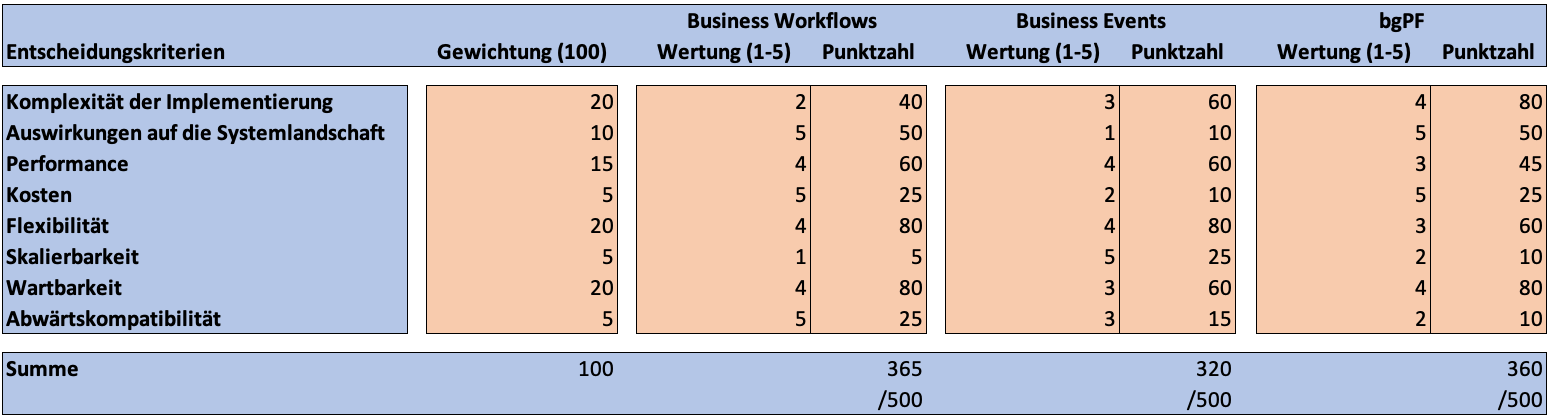
\includegraphics[height=4.06cm]{Bilder/Handlungsempfehlung_Entscheidungsmatrix.png}
%  \caption[gewichtete Entscheidungsmatrix der drei Ansätze]{gewichtete Entscheidungsmatrix der drei Ansätze, eigene Darstellung}
%  \label{fig:iso_norm}
% \end{figure}

\begin{table}[h]
    \centering
    \begin{tabular}{c}
        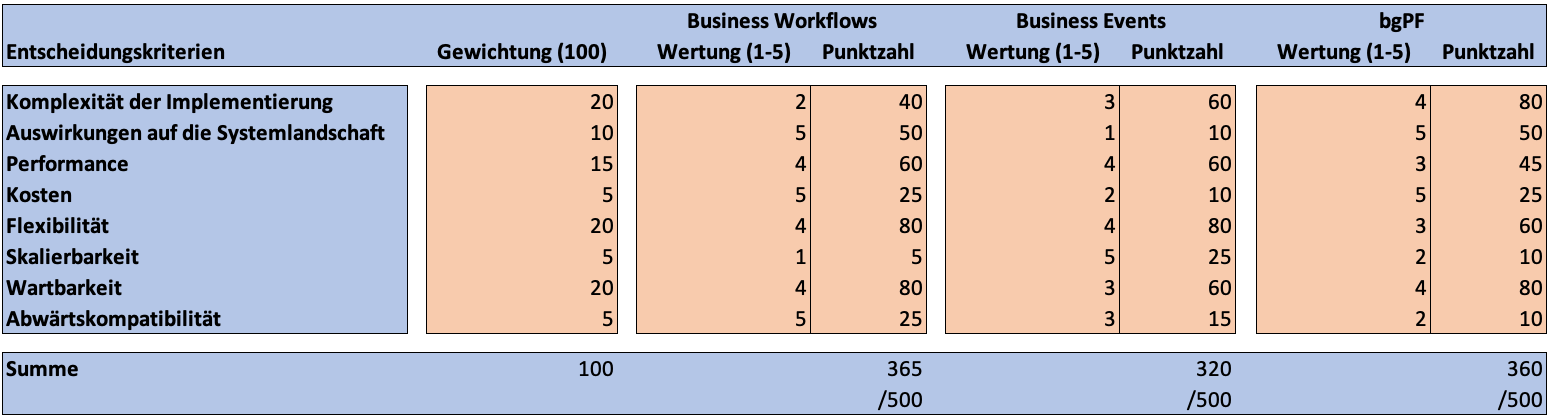
\includegraphics[height=4cm]{Bilder/Handlungsempfehlung_Entscheidungsmatrix.png}
    \end{tabular}
    \caption[Gewichtete Entscheidungsmatrix der drei Ansätze]{Gewichtete Entscheidungsmatrix der drei Ansätze. Eigene Darstellung}
    \label{tab:iso_norm_Entscheidungsmatrix}
\end{table}


Die Gewichtungen der Kriterien wurden durch eine abteilungsinterne Befragung der für das Thema verantwortlichen Personen ermittelt. Die Wertungen der Technologien für die einzelnen Vergleichspunkte wurden aus dem Vergleich im vorhergehenden Kapitel bestimmt. Somit ergibt sich, dass die Technologie Business Workflows, die auch aktuell zum Lösen der Problemstellung im Betrieb zum Einsatz kommt tatsächlich, entgegen der anfänglichen Annahme die beste Variante ist, wenn auch der Unterschied zum bgPF nur sehr marginal ist (Vgl. Abb. \ref{fig:iso_norm_Diagramm}). Da die Bewertungen relativ zueinander erfolgt sind, bei den beiden Technologien nur um 1\% abweichen und generell ähnliche Stärken haben, sollten diese als gleichwertig geeignet für die Lösung der Problemstellung betrachtet werden. Business Events würden sich zwar grundlegend auch für den Anwendungsfall eigenen, bieten aber insgesamt nicht so viele Vorteile wie die anderen beiden Ansätze. Allgemein hängt die Wahl von der spezifischen Gewichtung der einzelnen Kriterien ab. 

\section{Reflexion der Arbeit und Ausblick}

Die anfängliche Fragestellung der Arbeit war, welcher der drei vorgestellten Lösungsansätze am besten im betrieblichen Anwendungsszenario eingesetzt werden sollte und welcher Ansatz sich allgemein anhand mehrerer Vergleichskriterien wofür eignet. Im letzten Kapitel des Praxisteils und im vorhergehenden Kapitel der Arbeit wurden diese Fragen nun beantwortet. Es wurde gezeigt welcher Ansatz für die Abteilung der geeignetste wäre sowie allgemein die Stärken und Schwächen der einzelnen Ansätze herausgestellt, sodass die Ergebnisse ohne Weiteres auch auf andere ähnliche Szenarien übertragen werden können. Möglichkeiten der weitergehenden Forschung bestehen vor allem darin, die vorgestellten Ansätze anhand von Prototypen oder Proof-of-Concepts in der Praxis anzuwenden und somit auch eine praktische Referenz für die Umsetzung sequentieller Prozesse im RESTful-API Umfeld mit einem transaktionalen Kontext zu bilden. Des Weiteren können auch noch weitere Ansätze zur Umsetzung solcher Prozesse betrachtet werden, die in dieser Arbeit aufgrund des Umfangs keine Berücksichtigung finden konnten.